\documentclass[../main-physics-problems.tex]{subfiles}
\begin{document}

\subsection{Physical Systems}

\subsubsection{Choices for a System}
\subsubsection{Energy Stored in the Arrangement of Particles}
\clearpage

\subsubsection{Gravitational and Elastic Potential Energy}

\begin{questions}
\question
Recall Newton's universal law of gravitation:

\begin{equation*}
    F_g = \frac{G m_1 m_2}{r^2}
\end{equation*}

where $G = \SI{6.67e-11}{N\cdot m^2/kg^2}$. Calculate the gravitational force by Earth on a 1.0 kilogram object resting on the surface of Earth. Earth's mass is \SI{5.97e24}{kg}, and the separation distance between Earth and object is Earth's radius, \SI{6.378e8}{m}.

\question
When two masses are separated by some distance, in addition to a mutual force of attraction, there is energy stored in the configuration; we call it gravitational potential energy $E_g$:

\bigskip

\begin{minipage}{0.4\textwidth}
\Large 
\begin{equation*}
    E_g = -\frac{G m_1 m_2}{r}
\end{equation*}
\end{minipage}%
\begin{minipage}{0.4\textwidth}
\centering
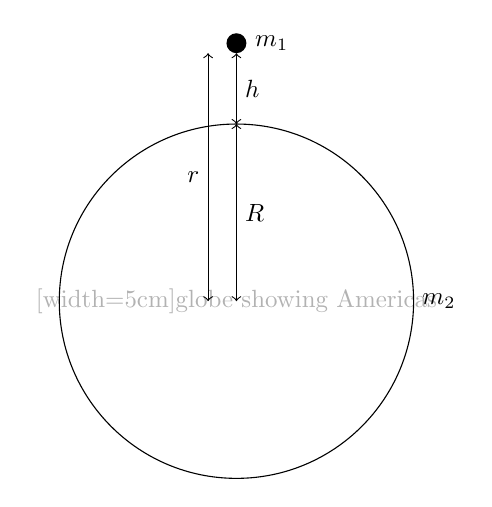
\begin{tikzpicture}[scale=0.9,transform shape]
    \draw (0,0) node[opacity=0.3] {\twemoji[width=5cm]{globe showing Americas}};
    \draw (0,0) circle (2.5) node[right=2.5cm] {$m_2$};
    \draw[<->] (0,0) -- (0,2.5) node[right,pos=0.5] {$R$};
    \draw[<->,xshift=-4mm] (0,0) -- (0,3.5) node[left,pos=0.5] {$r$};
    \begin{scope}[shift={(0,2.5)}]
        \draw[<->] (0,0) -- (0,1) node[right,pos=0.5] {$h$};
        \fill[yshift=4pt] (0,1) circle (4pt) node[right=4pt] {$m_1$};
    \end{scope}
\end{tikzpicture}

\underline{Note:} Figure not to scale.
\end{minipage}

\bigskip


Go to \href{https://www.desmos.com/scientific}{desmos.com/scientific}. Define the following variables in each cell:
\vspace{-1em}

\begin{align*}
    & G = \num{6.8139e-11} \\[1ex]
    & m_1 = 1.00 \\[1ex]
    & m_2 = \num{5.97e24} \\[1ex]
    & R = \num{6.378e6} \\[1ex]
    & h = 0 
\end{align*}

where $G$ is a slightly modified\footnote{Setting $G = \num{6.814e-11}$ makes $g = 10$.} version of the universal gravitational constant, $m_1$ is a test mass (like a bowling ball), $m_2$ is the mass of the Earth in kilograms, $r$ is the Earth's radius in meters, and $h$ is the vertical position of the object relative to the surface of the Earth (i.e., the height above ground). 

Next, define the initial and final gravitational potential energy between the Earth and test mass as

\begin{align*}
    E_i &= -\frac{G m_1 m_2}{R} \\[1ex]
    E_f &= - \frac{G m_1 m_2}{R+h}
\end{align*}

where the term $r+h$ represents the Earth's radius plus the height to which the object has been raised.

Finally, define the \textit{change} in gravitational potential energy as

\begin{equation*}
    E_{\mathrm{change}} = E_f - E_i
\end{equation*}

\begin{parts}
\part Set the object position to $h = 0$, and list the initial, final, and change in gravitational potential energies below:

\begin{center}
\bgroup
\def\arraystretch{1.5}
\begin{tabular}{|c|c|c|}
    \hline 
     \hspace{2.0cm} $E_i$ \hspace{2.0cm} & \hspace{2.0cm} $E_f$ \hspace{2.0cm} & \hspace{1cm} $E_\mathrm{change}$ \hspace{1.5cm} \phantom{.}\\ \hline
     \ifprintanswers \color{red} $-63780155$ \fi & \ifprintanswers \color{red} $-63780155$ \fi & \ifprintanswers \color{red} $0.00$ \fi \\ \hline
\end{tabular}
\egroup
\end{center}

\part 
Now set $h = 1$, and list the energies below.

\begin{center}
\bgroup
\def\arraystretch{1.5}
\begin{tabular}{|c|c|c|}
    \hline 
     \hspace{2.0cm} $E_i$ \hspace{2.0cm} & \hspace{2.0cm} $E_f$ \hspace{2.0cm} & \hspace{1cm} $E_\mathrm{change}$ \hspace{1.5cm} \phantom{.}\\ \hline
     \ifprintanswers \color{red} $-63780155$ \fi & \ifprintanswers \color{red} $-63780145$ \fi & \ifprintanswers \color{red} $+10.00$ \fi \\ \hline
\end{tabular}
\egroup
\end{center}

\part 
Now set $h = 2$, and list the energies below.

\begin{center}
\bgroup
\def\arraystretch{1.5}
\begin{tabular}{|c|c|c|}
    \hline 
     \hspace{2.0cm} $E_i$ \hspace{2.0cm} & \hspace{2.0cm} $E_f$ \hspace{2.0cm} & \hspace{1cm} $E_\mathrm{change}$ \hspace{1.5cm} \phantom{.}\\ \hline
     \ifprintanswers \color{red} $-63780155$ \fi & \ifprintanswers \color{red} $-63780135$ \fi & \ifprintanswers \color{red} $+20.00$ \fi \\ \hline
\end{tabular}
\egroup
\end{center}


\part 
Change test mass $m_1$ and vertical position $h$ according to the following tables and record the change in gravitational potential energy, $E_\mathrm{change}$, in each case.

\begin{center}
\bgroup
\def\arraystretch{2}
\begin{tabular}{|c|c|c|}
    \hline
    $m_1$ & $h$ & $E_\mathrm{change}$ \\ \hline
     1 & 0 & \ifprintanswers \textcolor{red}{0} \fi \\ \hline
     1 & 1 & \ifprintanswers \textcolor{red}{10} \fi \\ \hline
     1 & 2 & \ifprintanswers \textcolor{red}{20} \fi \\ \hline
     1 & 3 & \ifprintanswers \textcolor{red}{30} \fi \\ \hline
     1 & 4 & \ifprintanswers \textcolor{red}{40} \fi \\ \hline
     1 & 5 & \ifprintanswers \textcolor{red}{50} \fi \\ \hline
\end{tabular}%
\hspace{1cm}
\begin{tabular}{|c|c|c|}
    \hline
    $m_1$ & $h$ & $E_\mathrm{change}$ \\ \hline
     2 & 0 & \ifprintanswers \textcolor{red}{0} \fi \\ \hline
     2 & 1 & \ifprintanswers \textcolor{red}{20} \fi \\ \hline
     2 & 2 & \ifprintanswers \textcolor{red}{40} \fi \\ \hline
     2 & 3 & \ifprintanswers \textcolor{red}{60} \fi \\ \hline
     2 & 4 & \ifprintanswers \textcolor{red}{80} \fi \\ \hline
     2 & 5 & \ifprintanswers \textcolor{red}{100} \fi \\ \hline
\end{tabular}%
\hspace{1cm}
\begin{tabular}{|c|c|c|}
    \hline
    $m_1$ & $h$ & $E_\mathrm{change}$ \\ \hline
     3 & 0 & \ifprintanswers \textcolor{red}{0} \fi \\ \hline
     3 & 1 & \ifprintanswers \textcolor{red}{30} \fi \\ \hline
     3 & 2 & \ifprintanswers \textcolor{red}{60} \fi \\ \hline
     3 & 3 & \ifprintanswers \textcolor{red}{90} \fi \\ \hline
     3 & 4 & \ifprintanswers \textcolor{red}{120} \fi \\ \hline
     3 & 5 & \ifprintanswers \textcolor{red}{150} \fi \\ \hline
\end{tabular}
\egroup
\end{center}

\part \textit{Synthesis.} Look at the patterns in your data table and think about the mathematical relationship between mass $m_1$, height $h$, and change in gravitational potential energy $E_\mathrm{change}$. Then make a prediction for the equation for $E_\mathrm{change}$ in terms of $m_1$ and $h$.

\bgroup
\Large
\begin{equation*}
    E_\mathrm{change} = \ifprintanswers \color{red} \else \color{white} \fi mh \times 10 = mgh
\end{equation*}
\egroup

\part
In words, express the equation you developed in the previous step. Start your sentence as, ``The change in gravitational potential energy equals \dots ''

\ifprintanswers
{\color{red} The change in gravitational potential energy equals mass multiplied by height multiplied by 10; or mass multiplied by the acceleration due to gravity multiplied by height.}
\else
\fillwithlines{1.5cm}
\fi
\end{parts}

\clearpage

\question
Let $h_0$ be a variable reference point above Earth's surface from which we may measure a change in gravitational potential energy. 

\begin{center}
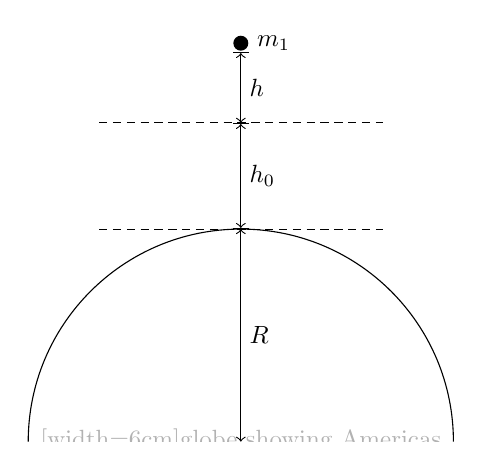
\begin{tikzpicture}[scale=0.9,transform shape]
    \begin{scope}
        \clip (-3,0) -- (3,0) arc (0:180:3);
        \draw (0,0) node[opacity=0.3] {\twemoji[width=6cm]{globe showing Americas}};
    \end{scope}
    \draw (3,0) arc (0:180:3);
    \draw[densely dashed] (-2,3) -- (2,3);
    \draw[densely dashed] (-2,4.5) -- (2,4.5);
    \draw[<->] (0,0) -- (0,3) node[right,pos=0.5] {$R$};
    \draw[|<->|] (0,3) -- (0,4.5) node[right,pos=0.5] {$h_0$};
    \draw[<->|] (0,4.5) -- (0,5.5) node[right,pos=0.5] {$h$};
    \fill[yshift=3.5pt] (0,5.5) circle (3pt) node[right=3pt] {$m_1$};
\end{tikzpicture}
\end{center}

For example, if the reference point is at sea level, then $h_0 = \SI{0}{m}$; if it's at the top of a 100-meter building, then $h_0 = \SI{100}{m}$; etc. Then update the cells for the initial and final gravitational potential energies as

\begin{align*}
    E_i &= -\frac{G m_1 m_2}{R + h_0} \\[1ex]
    E_f &= - \frac{G m_1 m_2}{R + h_0 + h}
\end{align*}

\begin{parts}
\part The tallest building in Houston, the JP Morgan Chase Tower, is 305 meters tall. Houston is 15 meters above sea level. So, let's set the reference point at the top of the building, at $h_0 = 320$. Calculate the change in gravitational potential energy when $m_1$ is raised $h=10$ meters above the reference point.

\bigskip

$E_\mathrm{change} = $ \fillin[10.00]

\bigskip

Is the formula $\Delta E_g = mgh$ appropriate?

\part 
Mount Everest is \SI{8850}{m} above sea level. Set $h_0 = 8850$. 

\begin{center}
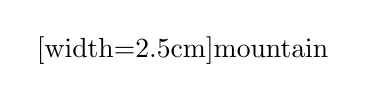
\begin{tikzpicture}
    \draw (0,0) node {\twemoji[width=2.5cm]{mountain}};
\end{tikzpicture}
\end{center}

Now what is the change in gravitational potential energy when $m_1$ is raised $h=10$ meters above the reference point?

\bigskip

$E_\mathrm{change} = $ \fillin[99.72]

\bigskip

Is the formula $\Delta E_g = mgh$ appropriate?

\part 
The International Space Station (ISS) orbits 400 kilometers above the surface of the Earth. Set the reference point at $h_0 = 400000$. What is the change in gravitational potential energy when $m_1$ is raised $h=10$ meters above the reference point?

\bigskip

$E_\mathrm{change} = $ \fillin[88.55]

\bigskip

Is the formula $\Delta E_g = mgh$ appropriate near the space station?

\end{parts}

\begin{center}
    
\end{center}

\question \label{xxSTEr}
What is the equation for gravitational potential energy? What is the SI unit of gravitational potential energy?


\question
What is the magnitude of acceleration due to gravity on Earth, $g$?


\question \label{9p9meZ}
Determine the gravitational potential energy gained by a 4.0-kg rock that is raised to a height of \SI{18.00}{m}.
%\correctchoice \SI{705.6}{J}

\begin{solution}
\SI{705.6}{J}
\end{solution}


\question \label{i6NTnH}
Spots, the leopard whose mass is \SI{55.0}{kg}, climbs 12.0 meters up a tree. What is Spots's gravitational potential energy relative to the ground?

\begin{solution}
\SI{6468}{J}
\end{solution}

\question \label{FAhPt5}
Santi, the soccer player, kicks a 2-kilogram ball up to a height of 15 meters. At this peak height, what is the ball's gravitational potential energy?

\begin{solution}
\SI{294}{J}
\end{solution}


\question \label{Nn51QC}
A 5-kilogram ball gets kicked in the air to a maximum height of 39 meters. At the peak, what is the ball's gravitational potential energy?

\begin{solution}
\SI{1911}{J}
\end{solution}

\textbf{\ref{4S1RQ9}--\ref{Y0v7pI}} Calculate gravitational potential energy.

\question \label{4S1RQ9}
Mass is \SI{15}{kg}. Height is \SI{12}{m}.

\begin{solution}
\SI{1764}{J}
\end{solution}


\question \label{NS8TFJ}
Mass is \SI{50}{kg}. Height is \SI{26}{m}.

\begin{solution}
\SI{1.27e4}{J}
\end{solution}


\question \label{29XPZj}
$m = \SI{9}{kg}$. $h = \SI{51}{m}$.

\begin{solution}
\SI{4498}{J}
\end{solution}


\question \label{Fv0opf}
$m = \SI{87}{kg}$. $h = \SI{2}{m}$.

\begin{solution}
\SI{1705}{J}
\end{solution}


\question \label{Y0v7pI}
Mass is 2000 kilograms. Height is 3 kilometers.

\begin{solution}
\SI{5.88e7}{J}
\end{solution}


\question \label{CdBjWD}
Milo, the \SI{4.5}{kg} cat, while attempting to catch a fly on the wall, leaps as high as he can and gains \SI{66.15}{J} of gravitational potential energy. How high did Milo jump?

\begin{solution}
\SI{1.5}{m}
\end{solution}


\question \label{M8oc7x}
How high above the ground is an object with a mass of \SI{100}{kg} whose gravitational potential energy is \SI{49000}{J}?

\begin{solution}
\SI{50}{m}
\end{solution}

\question \label{4S3f3k}
A motorcycle gains 2.5 meters in height after riding off a ramp. If it's gravitational potential energy at that instant is \SI{9500}{J}, what is the motorcycle's mass?

\begin{solution}
\SI{387.8}{kg}
\end{solution}

\question \label{JangCo}
What is the mass of an object that has a gravitational potential energy of \SI{275}{J} when it is \SI{14}{m} above the ground?

\begin{solution}
\SI{2.0}{kg}
\end{solution}




\end{questions}


\subsubsection{Comparing Potential Energy}
\subsubsection{Multiple Representations for Total Mechanical Energy}

\begin{center}
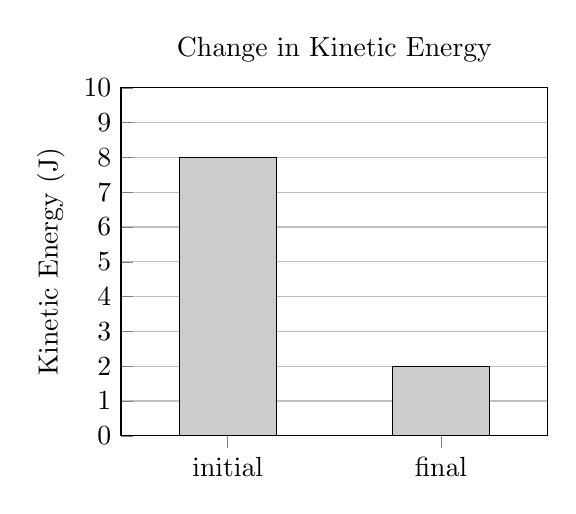
\begin{tikzpicture}
\begin{axis}[width=7cm,height=6cm,
    % axis lines=left,
    ybar,
    symbolic x coords={initial, final},
    xtick=data,
    ylabel={Kinetic Energy (J)},
    ymin=0, ymax=10,
    ytick={0,1,...,10},
    bar width=35pt,
    enlarge x limits=0.5,
    ymajorgrids=true,
    tick pos=left,
    title={Change in Kinetic Energy}
]
\addplot[black,fill=black!20] coordinates {(initial,8) (final,2)};
\end{axis}
\end{tikzpicture}
\end{center}

\subsubsection{Effects of Changing Physical Quantities on Energy}
\subsubsection{Calculations of Total Mechanical Energy}

\begin{questions}
\question
Suppose a 1-kilogram object is launched vertically upwards at \SI{18}{m/s}. Make a graph of the object's kinetic energy vs. time, gravitational potential energy vs. time, and total mechanical energy vs. time, as follows. Go to \href{https://www.desmos.com/calculator}{desmos.com/calculator}. Enter the following variables and equations in each cell:

\begin{align*}
    & m = 1 \\[1ex]
    & g = 10 \\[1ex]
    & v_0 = 18 \\[1ex]
    & v(t) = v_0 - gt \\[1ex]
    & K(t) = \frac{1}{2} m v\left(t\right)^2 \\[1ex]
    & h(t) = v_0 t - \frac{1}{2}g t^2 \\[1ex]
    & P(t) = mg h(t) \\[1ex]
    & E(t) = K(t) + P(t)
\end{align*}

where $m$ is mass, $g$ is gravitational acceleration, $v_0$ is the initial speed, $v(t)$ is the velocity as a function of time $t$, $K(t)$ is kinetic energy as a function of time, $h(t)$ is the vertical displacement, $P(t)$ is gravitational potential energy, and $E(t)$ is total mechanical energy.

\textbf{Disable} the graphs for $v(t)$ and $h(t)$ so that only $K(t)$, $P(t)$, and $E(t)$ are visible. Then click the graph settings (\faWrench) and set the X-Axis and Y-Axis limits to

\begin{equation*}
    0 \leq x \leq 4 \qquad \text{and} \qquad
    0 \leq y \leq 180
\end{equation*}

Finally, sketch the kinetic energy, gravitational potential energy, and mechanical energy vs. time graphs in the space below.

\begin{center}
\begin{tikzpicture}
\begin{axis}[height=6cm,width=8cm,
    axis lines=left,
    ylabel={Energy (J)},
    xlabel={Time (s)},
    ymin=0,ymax=180,
    xmin=0,xmax=4,
    ytick={0,20,...,180},
    xtick={0,0.5,...,4},
    % minor y tick num=1,
    % minor x tick num=1,
    grid=both,
]
    \ifprintanswers
    \addplot[domain=0:3.6,thick,variable=t,red] {0.5*1*(18-10*t)^2};
    \addplot[domain=0:3.6,thick,variable=t,green!50!black] {1*10*(18*t-0.5*10*t^2)};
    \addplot[domain=0:3.6,thick,variable=t] {0.5*1*(18-10*t)^2 + 1*10*(18*t-0.5*10*t^2)};
    \fi
\end{axis}
\end{tikzpicture}
\end{center}


\question \label{2EkX0c}
Define mechanical energy.




\end{questions}

\clearpage

\subsection{Energy is Conserved}

\subsubsection{Energy of a System Before and After an Event}

\subsubsection{Law of Conservation of Energy}

\begin{questions}

\question 
\href{https://phet.colorado.edu/en/simulations/energy-forms-and-changes}{Click here} to access the \texttt[red]{PhET Simulation: Energy Forms and Changes} (or Google it). Press the play ({\tiny \faPlay}) button in the center of the page. Click the \texttt[red]{Systems} panel. Check the \texttt[red]{Energy Symbols} box in the upper right-hand corner. Slide the slider under the bicycle to the right, remembering to periodically feed the cyclist, whom we will call Angelica. Answer Exercises \ref{UVgdHj}--\ref{IPOKOY} below.


\question \label{UVgdHj}
What are the 5 forms of energy shown in the simulation?


\question
What form of energy comes from within Angelica? (This is the energy she gets from food.)


\question
What form of energy does Angelica exert on the bike pedals?


\question
What form of energy is released by contact between the tire and the belt? 


\question
What form of energy causes the wooden turbine to rotate?


\question
The turbine coverts mechanical energy to what form of energy?


\question
Simulate a configuration in which light energy from the Sun gets transformed to electrical energy and then back to light energy (plus a bit of thermal energy). Draw a sketch of the final configuration and label the parts on your sketch.


\question
Simulate a configuration where energy transforms from light to electrical to mechanical energy. Draw a sketch of the configuration and label the parts.


\question
Simulate a configuration where energy transforms from thermal to mechanical to electrical and finally to light energy. Draw a sketch of the configuration and label the parts.


\question \label{IPOKOY}
Simulate a configuration where all 5 forms of energy are involved. Draw a sketch of the configuration and label all parts.

\question
Write the law of conservation of mechanical energy, both in words and in equation form. (There are 3 ways to write the equation.)


\question \label{kfZAyg}
Xena, the \SI{63}{kg} skateboarder, stars from rest from the top of a \SI{12}{m} parabolic ramp, like the one shown in Example \ref{mUfgIz}. What is her kinetic energy at the bottom of the ramp?

\begin{solution}
\SI{7408.9}{J}
\end{solution}


\question \label{5Nd1zt}
How fast is Xena, from Exercise \ref{kfZAyg}, going at the bottom of the ramp?

\begin{solution}
\SI{15.3}{m/s}
\end{solution}


\question \label{FWuV0W}
A 1.25-kg bowling ball is dropped from the top of the \href{https://en.wikipedia.org/wiki/JPMorgan_Chase_Tower_(Houston)}{JPMorgan Chase Tower}, the tallest building in Houston and in Texas. (Don't worry: all people and objects were safely cleared out below.) What is the kinetic energy of the bowling ball the instant before it impacts the ground? Assume there is no air resistance.

\begin{solution}
\SI{3741}{J}
\end{solution}

\question \label{c4eP75}
Calculate the speed of the bowling ball from Exercise \ref{FWuV0W} the instant before it hits the ground.

\begin{solution}
\ref{c4eP75}. \SI{77.37}{m/s}
\end{solution}

\question
Imagine a ball on a track starts from rest at the position labeled \texttt{start} and moves down the track towards other positions. Assume no energy is transferred between the ball and the track or between the ball and the air around it. What is the highest position the ball will reach before stopping and going back down the track? 

\begin{center}
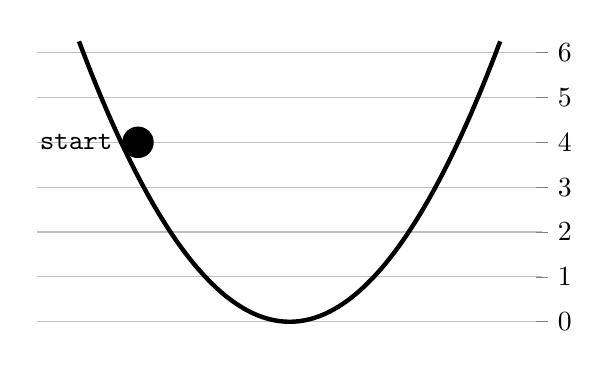
\begin{tikzpicture}
\begin{axis}[width=8cm,height=5cm,
    clip=false,
    xmin=-3,xmax=3,ymin=0,ymax=6,
    axis lines=right,
    axis line style={draw=none},
    %ticks=none,
    xtick style={draw=none},
    xticklabels={,,},
    ymajorgrids=true,
    ytick={0,1,...,6},
]

\addplot[ultra thick,samples=100,
    domain=-2.5:2.5
]{x^2}; 
\fill (-2*0.9,4) circle (2mm) node[left=2mm] {\texttt{start}};

\end{axis}
\end{tikzpicture}
\end{center}

\begin{randomizechoices}[keeplast]
    \correctchoice 4
    \choice 3
    \choice 2
    \choice 5
    \choice None of the above
\end{randomizechoices}



\question
A \SI{12.5}{kg} glider is observed flying at an altitude of \SI{1510}{m} at a constant velocity of \SI{18}{m/s}. The glider dives to a new altitude of \SI{1250}{m}. Neglecting the effects of air resistance, what is the change in the glider's gravitational potential energy?

\begin{randomizechoices}
\choice \SI{338000}{J}
\choice \SI{185000}{J}
\correctchoice \SI{-31850}{J}
\choice \SI{-15300}{J}
\end{randomizechoices}

\question
A diver with a mass of \SI{80.0}{kg} dives off a \SI{10.0}{m} platform. His velocity just before striking the water is \SI{14.0}{m/s}. What is his kinetic energy at that moment?

\begin{randomizechoices}
\choice \SI{800}{m/s}
\choice \SI{8000}{m/s}
\correctchoice \SI{7840}{m/s}
\choice \SI{7500}{m/s}
\end{randomizechoices}

\question
A ball is dropped from the top of a tall cliff. As the ball falls freely (without air resistance) toward the ground, its total mechanical energy\ldots 

\begin{randomizechoices}
\choice increases.
\choice decreases.
\correctchoice remains the same.
\end{randomizechoices}

\question
Using ground level as the reference height with zero potential energy, which object has the GREATEST gravitational potential energy?

\begin{randomizechoices}
\choice a \SI{40}{kg} object at a \SI{2}{m} height
\choice a \SI{2}{kg} object at a \SI{60}{m} height
\choice a \SI{5}{kg} object at a \SI{5}{m} height
\correctchoice a \SI{20}{kg} object at a \SI{50}{m} height
\end{randomizechoices}

\question
What is the kinetic energy of a \SI{2.0}{kg} toy car moving at \SI{5}{m/s}?

\begin{randomizechoices}
\choice \SI{10}{J}
\correctchoice \SI{25}{J}
\choice \SI{50}{J}
\choice \SI{5}{J}
\end{randomizechoices}

\question
How high can a worker on a construction crane lift a \SI{40}{kg} bag of sand if the crane uses \SI{4,000}{J} of energy? Assume no energy is used to overcome friction.

\begin{randomizechoices}
\choice \SI{160000}{m}
\choice \SI{1020}{m}
\correctchoice \SI{10.2}{m}
\choice \SI{16.0}{m}
\end{randomizechoices}

\question
Three hikers take three different paths to the top of a mountain, Paths 1, 2, and 3. The hikers are all have the same height and weight. When all of the hikers are at the finish point at the top of the mountain, which hiker will have the greatest amount of gravitational potential energy?

\begin{randomizechoices}
\choice The hiker who took Path 1. 
\choice The hiker who took Path 2.
\choice The hiker who took Path 3.
\choice The gravitational potential energy is the same for all the hikers.
\end{randomizechoices}

\question
A high diver steps off a diving platform that is 10 meters above the water. Assume there is no air resistance. During the fall, there will be a decrease in the diver's \fillin\ .

\begin{randomizechoices}
\choice kinetic energy
\choice total mechanical energy
\correctchoice gravitational potential energy
\choice momentum
\end{randomizechoices}


\question
The amount of potential energy possessed by an elevated object is equal to \fillin\ .

\begin{randomizechoices}
\choice the distance it is lifted
\choice the power used to lift it
\correctchoice the work done in lifting it
\choice the force needed to lift it
\choice the value of the acceleration due to gravity
\end{randomizechoices}

\question
A  ball is thrown into the air with \SI{100}{J} of kinetic energy, which is transformed to gravitational potential energy at the top of its trajectory. When it returns to its original level (neglecting air resistance), its kinetic energy is \fillin\ .

\begin{randomizechoices}
\choice less than \SI{100}{J}
\choice more than \SI{100}{J}
\correctchoice \SI{100}{J}
\choice not possible to calculate
\end{randomizechoices}

\question
An object that has kinetic energy must be \fillin\ .

\begin{randomizechoices}
\correctchoice moving
\choice at rest
\choice falling
\choice elevated
\end{randomizechoices}


\question
Mechanical energy can be in the form of

\begin{randomizechoices}
\choice kinetic energy only
\choice neither kinetic nor potential energy
\correctchoice both kinetic and potential energy
\choice potential energy only
\end{randomizechoices}

\question
Gravitational potential energy is the energy an object has stored due to its \fillin\ .

\begin{randomizechoices}
\choice density
\correctchoice height above ground
\choice color
\choice speed and direction
\end{randomizechoices}


\end{questions}

\subsubsection{Power (Revisited)}

\begin{questions}
\question
The SI unit of power is the \fillin\ .

\begin{randomizechoices}
\choice meter (m)
\choice joule (J)
\correctchoice watt (W)
\choice second (s)
\choice newton (N)
\end{randomizechoices}


\question
How much power is required to do \SI{40}{J} of work on an object in 5 seconds?

\begin{randomizechoices}
\choice \SI{200}{W}
\choice \SI{5}{W}
\choice \SI{40}{W}
\choice \SI{0}{W}
\correctchoice \SI{8}{W}
\end{randomizechoices}

\question
How much power is expended if you lift a \SI{60}{N} crate 10 meters in 1 second?

\begin{randomizechoices}
\choice \SI{6}{W}
\choice \SI{0}{W}
\correctchoice \SI{600}{W}
\choice \SI{10}{W}
\choice \SI{60}{W}
\end{randomizechoices}
\end{questions}

\clearpage

\subsection{Momentum is Conserved}

\subsubsection{Momentum, Force, and Impulse in Collisions and Explosions}

\subsubsection{Total Momentum Before and After Collisions and Explosions}

\subsubsection{Law of Conservation of Momentum}

\begin{questions}
\question
State the law of conservation of momentum.


\question
When is momentum said to be conserved?


\question
What is an isolated system?


\question
A ball is hit by a racket and its momentum changes. Under what conditions is momentum conserved?
\end{questions}

\subsubsection{Solving for Unknown Quantities using Conservation of Momentum}


\begin{questions}



\question \label{yEzMEO}
A billiards ball rolling on the table has momentum $p_1$. It hits another stationary ball, which then starts rolling. Considering friction to be negligible, what will happen to the momentum of the first ball?

\begin{solution}
It will decrease.
\end{solution}

\question
Give an example of an isolated system. (\textit{Hint}: What were some of the examples alluded to in the text?)


\question \label{Fl5xyW}
As in Example \ref{W5BnBq}, calculate the recoil velocity of an 85-kilogram man who, standing on a frictionless surface, throws a \SI{20}{kg} boulder away from his body at \SI{6.0}{m/s}.

\begin{solution}
\SI{-1.4}{m/s}
\end{solution}


\question \label{dMW612}
Solve Example \ref{W5BnBq} without plugging in the given numbers; that is, by algebraically manipulating the variables only. Your final answer should be an equation for $v_1^{\prime}$ in terms of $m_2$, $v_2^{\prime}$, and $m_1$.

\begin{solution}
$v_1^{\prime} = -\frac{m_2\,v_2^{\prime}}{m_1}$
\end{solution}
%%%%%%%%

\question \label{rhrGbz}
What is an elastic collision?


% \question
%     In which type of collision is kinetic energy conserved?
% 

\question\label{bTj1d8} %%% I made a mistake creating this problem. Need to fix this problem to ensure it doesn't violate conservation of energy. 
An object with a mass of \SI{7.0}{kg} moving at \SI{13.6}{m/s} experiences an elastic collision with an object of mass \SI{23}{kg} moving at \SI{-1.9}{m/s}. The first object's velocity after collision is \SI{-2.5}{m/s}. Draw a sketch with labels, like the one shown in Example \ref{wXY1rT}, and calculate the second object's velocity after collision.

\begin{solution}
\SI{3.0}{m/s}
\end{solution}


\question \label{O4Og7L} %%% I made a mistake creating this problem. Need to fix this problem to ensure it doesn't violate conservation of energy. 
Mass of the first object is \SI{2.0}{kg}.
Initial velocity of the first object is \SI{10}{m/s}. 
Mass of the second object is \SI{6.0}{kg}. 
Initial velocity of the second object is \SI{-1.5}{m/s}. 
Velocity of the first object after collision is \SI{-3}{m/s}.

\begin{solution}
\SI{2.83}{m/s}
\end{solution}

\question \label{6yR4Xo} %%% I made a mistake creating this problem. Need to fix this problem to ensure it doesn't violate conservation of energy. 
Mass of the first object is \SI{354}{kg}.
Initial velocity of the first object is \SI{58}{m/s}. 
Mass of the second object is \SI{768}{kg}. 
Initial velocity of the second object is \SI{-47}{m/s}. 
Velocity of the first object after collision is \SI{-20}{m/s}.

\begin{solution}
\SI{-11.0}{m/s}
\end{solution}



\question \label{Hjk6xk}
What is an inelastic collision?


\question \label{3Fptzi}
An object with a mass of \SI{1.25}{kg} moving at a velocity of \SI{2.11}{m/s} experiences an inelastic collision with a \SI{3.00}{kg} object that is moving at \SI{-1.90}{m/s}. Draw a sketch of the objects, including given and unknown quantities, like the figure in Example \ref{usQeew}. What is the final velocity of the combined system after the collision, $v^{\prime}$? 

\begin{solution}
\SI{-0.72}{m/s}
\end{solution}


\question \label{17GLnY}
In which direction does the system in Exercise \ref{3Fptzi} above move after the collision?

\begin{solution}
To the left
\end{solution}


\question \label{yJLtfh}
A \SI{604}{kg} object that is moving at a velocity of \SI{21.0}{m/s} inelastically collides with a \SI{934}{kg} object that is moving at \SI{-8.31}{m/s}. What is the final velocity of the combined system after the collision?

\begin{solution}
\SI{3.20}{m/s}
\end{solution}


\question \label{ViY0SX}
In which direction does the system in Exercise \ref{yJLtfh} above move after the collision?

\begin{solution}
To the right
\end{solution}


\question \label{jA5zHj}
Find the magnitude of the recoil velocity of a \SI{65}{kg} ice hockey goalie who catches a \SI{0.15}{kg} hockey puck slapped at him at a velocity of \SI{53}{m/s}. Assume that the goalie is at rest before catching the puck, and that friction between the ice and the puck-goalie system is negligible.

\begin{solution}
\SI{0.12}{m/s}
\end{solution}





% Joules and \href{https://www.cancer.gov/sites/g/files/xnrzdm211/files/styles/cgov_enlarged/public/cgov_image/media_image/2020-05/changes-nutrition-facts-label.jpg?h=54378ca5&itok=zYh4n-kk}{Calories} are the same type of unit: they measure energy.








\clearpage

\question
What is momentum?

\begin{randomizechoices}
\choice The product of a system's net force and time.
\choice The product of a system's mass and change in velocity.
\correctchoice The product of system's mass and velocity.
\choice The product of a system's mass and acceleration.
\end{randomizechoices}

\question
A \SI{70}{kg} skier leaves a ski jump at a velocity of \SI{14}{m/s}. What is the skier's momentum at that instant?

\begin{randomizechoices}
\choice \SI{50}{kg\,m/s}
\choice \SI{9800}{kg\,m/s}
\correctchoice \SI{980}{kg\,m/s}
\choice \SI{5}{kg\,m/s}
\end{randomizechoices}

\question
A child on a sled moves down a hill at 20 meters per second. The combined mass of the child-sled system is 100 kilograms. What is the momentum of the system?

\begin{randomizechoices}
\choice \SI{20}{kg\,m/s}
\correctchoice \SI{2000}{kg\,m/s}
\choice \SI{5}{kg\,m/s}
\choice \SI{1000}{kg\,m/s}
\end{randomizechoices}

\question
Which of the following vehicles has the greatest momentum?

\begin{randomizechoices}
\correctchoice a car with a mass of \SI{1210}{kg} moving at a velocity of \SI{51}{m/s}
\choice a truck with a mass of \SI{6120}{kg} moving at a velocity of \SI{10}{m/s}
\choice a car with a mass of \SI{1540}{kg} moving at a velocity of \SI{38}{m/s}
\choice a truck with a mass of \SI{2250}{kg} moving at a velocity of \SI{25}{m/s}
\end{randomizechoices}

\question
A ball is hit with a bat. A student determines that the momentum of the ball is \SI{1.0}{kg\,m/s}. If the ball's velocity is 2.0 meters per second, what is the ball's mass?

\begin{randomizechoices}
\choice \SI{1.0}{kg}
\choice \SI{2.0}{kg}
\correctchoice \SI{0.5}{kg}
\choice \SI{0.0}{kg}
\end{randomizechoices}

\question
Freddy, the \SI{2.0}{kg} fish, travels through the Pacific Ocean at a velocity of \SI{5.0}{m/s} when a temporary force causes Freddy to slow down to a velocity of \SI{2.0}{m/s}. What is Freddy's change in momentum?

\begin{randomizechoices}
\choice \SI{6.0}{kg\,m/s}
\choice \SI{3.0}{kg\,m/s}
\correctchoice \SI{-6.0}{kg\,m/s}
\choice \SI{-3.0}{kg\,m/s}
\end{randomizechoices}

\question
Robbie Ray throws a \SI{0.145}{kg} baseball at a velocity of \SI{-43}{m/s}, and Yordan Alvarez hits the ball back at \SI{37}{m/s}. Assuming the ball travels in one dimension only, what is the baseball's change in momentum?

\begin{randomizechoices}
\choice \SI{5.36}{kg\,m/s}
\choice \SI{6.23}{kg\,m/s}
\correctchoice \SI{11.6}{kg\,m/s}
\choice \SI{0.87}{kg\,m/s}
\end{randomizechoices}

\question
Impulse is the product of \fillin\ .

\begin{randomizechoices}
\choice mass and velocity ($mv$)
\choice mass and acceleration ($ma$)
\correctchoice net force and time ($F_{\text{net}}\,\Delta t$)
\choice net force and velocity ($F_{\text{net}}\,v$)
\end{randomizechoices}

\question
According to the impulse-momentum theorem, the impulse experienced by an object is equivalent to the object's \fillin\ .

\begin{randomizechoices}
\choice momentum
\correctchoice change in momentum
\choice velocity
\choice force
\end{randomizechoices}

% \question
% What is the impulse-momentum theorem in equation form?

% \begin{randomizechoices}
% \choice $p=mv$
% \choice $F_{\text{net}} = ma$
% \choice $\Delta p = m (v_f - v_i)$
% \correctchoice $\Delta p = F_{\text{net}}\,\Delta t$
% \end{randomizechoices}

% \question
% Which two quantities can be expressed using the same units?

% \begin{randomizechoices}
% \choice momentum and energy
% \correctchoice impulse and momentum
% \choice energy and force
% \choice force and impulse
% \end{randomizechoices}

\question
According to the impulse-momentum theorem, why is it that, if you fall off your roof, you will experience a lesser net force ($F_{\text{net}}$) when you land on a trampoline compared to when you land on the ground?

\begin{randomizechoices}
\choice The trampoline decreases the elapsed time ($\Delta t$) during which you come to a stop.
\correctchoice The trampoline increases the elapsed time ($\Delta t$) during which you come to a stop.
\choice The trampoline increases your change in momentum ($\Delta p$).
\choice The trampoline decreases your change in momentum ($\Delta p$).
\end{randomizechoices}

% \question
% An egg dropped on the road usually breaks, while one dropped on the grass usually does not break. The impulse-momentum theorem suggests that for the egg dropped on the grass 

% \begin{randomizechoices}
% \choice the time interval for stopping is less.
% \correctchoice the time interval for stopping is greater.
% \choice the change in momentum is greater.
% \choice the change in momentum is less.
% \end{randomizechoices}

\question
A ball is hit with a force of \SI{40}{N}. It is in contact with the bat for 0.02 seconds. What is the change in momentum of the ball?

\begin{randomizechoices}
\choice \SI{2000}{kg\,m/s}
\choice \SI{0.08}{kg\,m/s}
\choice \SI{8.0}{kg\,m/s}
\correctchoice \SI{0.8}{kg\,m/s}
\end{randomizechoices}

% \question
% What impulse will a \SI{25}{kg} cart experience if it starts at rest and accelerates to a speed of \SI{12}{m/s}?

% \begin{randomizechoices}
% \choice \SI{2.10}{N\,s}
% \correctchoice \SI{300}{N\,s}
% \choice \SI{0.48}{N\,s}
% \choice \SI{13.0}{N\,s}
% \end{randomizechoices}

% \question
% A \SI{0.45}{kg} football traveling at a speed of \SI{22}{m/s} is caught by an \SI{84}{kg} stationary receiver. If the football comes to rest in the receiver's arms, what is the magnitude of the impulse imparted on the ball by the receiver's hands?

% \begin{randomizechoices}
% \choice \SI{3.8}{N\,s}
% \choice \SI{4.4}{N\,s}
% \correctchoice \SI{9.9}{N\,s}
% \choice \SI{1800}{N\,s}
% \end{randomizechoices}

\question
The law of conservation of momentum states that

\begin{randomizechoices}
    \choice the total momentum of all objects interacting with one another is zero
    \correctchoice the total initial momentum of all objects before an interaction equals the total final momentum after the interaction
    \choice the total initial momentum of all objects interacting with one another does not equal the total final momentum  
    \choice the total initial momentum of all objects is zero 
\end{randomizechoices}

\clearpage
\question
Soccer ball 1 collides with soccer ball 2, which was at rest. The total momentum of the two-object system after the collision \fillin\ .

\begin{randomizechoices}
    \choice is zero
    \choice increases
    \correctchoice remains constant
    \choice decreases
\end{randomizechoices}

\question
A \SI{60}{kg} student on ice skates stands at rest on a frictionless frozen pond holding a \SI{10}{kg} brick. He throws the brick eastward with a speed of \SI{18}{m/s}. What is the student's recoil velocity?

\begin{randomizechoices}
\choice \SI{3.0}{m/s} east
\correctchoice \SI{3.0}{m/s} west
\choice \SI{18}{m/s} west
\choice \SI{18}{m/s} east
\end{randomizechoices}

\question
A \SI{1000}{kg} cannon fires a \SI{10}{kg} projectile horizontally at a velocity of \SI{300}{m/s}. What is the recoil velocity of the cannon?

\begin{randomizechoices}
\choice \SI{0.3}{m/s}
\correctchoice \SI{3.0}{m/s}
\choice \SI{300}{m/s}
\choice \SI{30}{m/s}
\end{randomizechoices}

\question
Two shopping carts stick together and move with the same velocity after colliding. This collision is \fillin\ one.

\begin{randomizechoices}
\choice an impulse
\correctchoice an inelastic
\choice an elastic
\choice a momentum
\end{randomizechoices}

\question
After two billiard balls collide, they veer off in different directions. This is \fillin\ collision.

\begin{randomizechoices}
\choice an impulse
\choice an inelastic
\correctchoice an elastic
\choice a momentum
\end{randomizechoices}

\question
A car is hit by a train. The car sticks to the front of the train and is dragged down the tracks. What type of collision is this?

\begin{randomizechoices}
\choice impulse
\choice elastic collision
\correctchoice inelastic collision
\choice momentum
\end{randomizechoices}

\clearpage


\begin{EnvUplevel}
\textbf{Questions \ref{SGv3JM} and \ref{jlNXIi}.} Two medicine balls elastically collide. Their masses and velocities before the collision are shown in the figure below.
\end{EnvUplevel}

\begin{center}
\def\xa{1.5}
\def\xb{8.5}
\def\y{3}
\def\rb{6mm}
\begin{tikzpicture}
\begin{axis}[width=8cm, height=3cm,
    ticks=none,
    axis line style={draw=none},
    clip=false,
    xmin=0,xmax=10,
    ymin=0,ymax=10,
]
    \draw[thick,->] (\xa,\y) -- ++(axis direction cs: 3,0) node[above] {$\SI{2.75}{m/s}$};
    \fill[black!15] (\xa-0.3,\y) circle (3mm);
    \fill[black!30] (\xa-0.15,\y) circle (3mm);
    \draw[fill=black] (\xa,\y) circle (3mm) node[below=3mm] {$\SI{2.00}{kg}$} node[above=3mm] {$m_1$};
    \fill[black!15] (\xb+0.3,\y) circle (\rb);
    \fill[black!30] (\xb+0.15,\y) circle (\rb);
    \draw[thick,->] (\xb,\y) -- ++(axis direction cs: -2.3,0) node[below] {$\SI{-1.00}{m/s}$};
    \draw[fill=black] (\xb,\y) circle (\rb) node[below=\rb] {$\SI{3.00}{kg}$} node[above=\rb] {$m_2$};
\end{axis}
\end{tikzpicture}
\end{center}

\question \label{SGv3JM}
If the first object's velocity after the collision is \SI{-1.75}{m/s}, how fast will the second ball move after the collision?

\begin{randomizechoices}
\choice \SI{1.00}{m/s}
\correctchoice \SI{2.00}{m/s} 
\choice \SI{1.75}{m/s}
\choice \SI{3.25}{m/s}
\end{randomizechoices}

\question \label{jlNXIi}
In which direction will the second ball travel after the collision?

\begin{randomizechoices}
\correctchoice right
\choice left
\choice no direction (it will stop moving)
\choice It's not possible to determine with the given information.
\end{randomizechoices}

\bigskip

\hrule

\begin{EnvUplevel}
\textbf{Questions \ref{first_question}--\ref{last_question}.} A \SI{32}{kg} object moving at \SI{6.7}{m/s} to the RIGHT collides with a \SI{220}{kg} object moving with a speed of \SI{5.9}{m/s} to the LEFT. The objects undergo an elastic collision.
\end{EnvUplevel}

\question \label{first_question}
 If after the collision the first object bounces backward with a speed of \SI{15.3}{m/s}, what is speed of the second object? (\textit{Hint}: Draw a sketch. Remember that velocity is speed AND direction, and speed does not indicate direction.)

\begin{randomizechoices}
\correctchoice \SI{2.7}{m/s}
\choice \SI{3.6}{m/s}
\choice \SI{0.0}{m/s}
\choice \SI{7.6}{m/s}
\end{randomizechoices}

 \question \label{last_question}
 In which direction does the second object move after the collision?

\begin{randomizechoices}
\correctchoice Left
\choice Right
\choice No direction (it stops moving).
\choice Up
\end{randomizechoices}

\bigskip

\hrule

\clearpage
\question
Each croquet ball in a set has a mass of \SI{0.50}{kg}. The \textbf{green} ball travels at \SI{10.5}{m/s} and strikes a stationary \textbf{red} ball. If the \textbf{green} ball stops moving after colliding with the \textbf{red} one, what is the final speed of the \textbf{red} ball after the collision?

\begin{randomizechoices}
\choice \SI{12.0}{m/s}
\choice \SI{9.6}{m/s}
\correctchoice \SI{10.5}{m/s}
\choice \SI{6.0}{m/s}
\end{randomizechoices}

\question 
Jennifer loads a shopping cart with \SI{75}{kg} of groceries. She launches the cart at \SI{15}{m/s} into another \SI{315}{kg} shopping cart that is initially at rest. The two carts stick together after the collision. What is the final velocity of the two-object system?

\begin{randomizechoices}
\correctchoice \SI{2.9}{m/s}
\choice \SI{12}{m/s}
\choice \SI{19}{m/s}
\choice \SI{3.6}{m/s}
\end{randomizechoices}

\bigskip

\hrule

\begin{EnvUplevel}
\textbf{Questions \ref{kfiru}--\ref{gR47a}.} Two football players undergo an inelastic collision. The figure below shows their masses and their velocities before the collision.
\end{EnvUplevel}


\begin{center}
\def\xa{1.5}
\def\xb{8.5}
\def\y{3}
\def\rb{6mm}
\begin{tikzpicture}
\begin{axis}[width=8cm, height=3cm,
    ticks=none,
    axis line style={draw=none},
    clip=false,
    xmin=0,xmax=10,
    ymin=0,ymax=10,
]
    \draw[thick,->] (\xa,\y) -- ++(axis direction cs: 3,0) node[above] {$\SI{7.23}{m/s}$};
    \fill[black!15] (\xa-0.3,\y) circle (3mm);
    \fill[black!30] (\xa-0.15,\y) circle (3mm);
    \draw[fill=black] (\xa,\y) circle (3mm) node[below=3mm] {$\SI{110}{kg}$} node[above=3mm] {$m_1$};
    \fill[black!15] (\xb+0.3,\y) circle (\rb);
    \fill[black!30] (\xb+0.15,\y) circle (\rb);
    \draw[thick,->] (\xb,\y) -- ++(axis direction cs: -2.2,0) node[below] {$\SI{-3.55}{m/s}$};
    \draw[fill=black] (\xb,\y) circle (\rb) node[below=\rb] {$\SI{135}{kg}$} node[above=\rb] {$m_2$};
\end{axis}
\end{tikzpicture}%
\end{center}

\question \label{kfiru}
At what speed is the combined system moving after the collision?

\begin{randomizechoices}
\correctchoice \SI{1.29}{m/s} 
\choice \SI{0.00}{m/s}
\choice \SI{3.68}{m/s}
\choice \SI{10.35}{m/s}
\end{randomizechoices}

\question \label{gR47a}
In what direction are the players moving after the collision?

\begin{randomizechoices}
\choice To the left.
\choice No direction: the players cancel each other's momentum.
\choice The law of conservation of momentum cannot indicate direction.
\correctchoice To the right.
\end{randomizechoices}

\bigskip

\hrule







\end{questions}

\end{document}